\chapter{Proof of Concept}
Nun wird das realisierte Konzept anhand der in Kapitel~\ref{scenarios} vorgestellten Fallstudien auf Applikabilität geprüft.
Aus den Ergebnissen dieses Kapitels kann im Anschluss ein Fazit gezogen und ein potentieller Ausblick auf künftige Erweiterungen des Konzepts gegeben werden.

\section{Von 3D Gebäudeplan zu Bauplanentwurf}
Zunächst müssen für Szenario 1 und 2 Gebäudepläne in einem Konstruktionsplaner modelliert werden.
Dazu wurde, wie schon in Kapitel~\ref{real:modellierung} beschrieben, die 3D Modellierungs-Software Blender herangezogen (siehe Kapitel~\ref{basics:blender}).
Diese kann mit der frei verfügbaren Erweiterung \textit{blenderbim} zu einem funktionsfähigen BIM Editor mit \textit{IFC} Unterstützung ausgebaut werden (auch diese Technologien wurden bereits in den Kapiteln~\ref{basics:blenderbim} und~\ref{basics:ifc} vorgestellt).
Darin lassen sich sowohl individuelle Wandtypen erstellen, als auch mithilfe der \textit{IfcProperties} Annotationen über Modul und Rastermaße daran anhängen.
Mit den in Kapitel~\ref{concept:raster} definierten Modellierungseinschränkungen, deren Umsetzung in Kapitel~\ref{real:modellierung} thematisiert wurde, konnte die Modellierungsphase sowohl erleichtert, als auch beschleunigt werden.

\subsection{Szenario 1}\label{poc:scenario1}
Die Modellierung der zwei sich in der Wanddicke unterscheidenden Versionen des 20 Meter hohen Turms mit einer Grundfläche von 10$\times$10 Metern in Blender war wenig komplex.
Es bedarf lediglich vier Wände, die einen quadratischen Raum bilden.
Das vollständige Gebäudemodell ist in Abbildung~\ref{fig:poc:scenario1 modell} zu sehen.
\begin{figure}[ht!]
  \centering
  
\includegraphics[width=0.6\columnwidth]{fig/TODO.jpg}
  \caption{TODO IFC Modell der beiden Türme.}\label{fig:poc:scenario1 modell}
\end{figure}
Das Ergebnis nach Anwenden der drei verschiedenen Mauerwerksverbände ist wie erwartet.
Die verschiedenen Verbände lassen sich wie in Kapitel~\ref{real:verband} gezeigt in den Programmcode einpflegen.
Das Basismodul ist überall dort zu sehen, wo ein gerader Wandabschnitt vorliegt.
Alle vier Eckbereiche sind korrekt identifiziert worden, denn dort wurde der für den jeweiligen Mauerwerksverband definierte Eckplan passend umgesetzt.
Im Falle des Kreuz- und Kopfverbandes wurde das Basismodul dabei etwas verkürzt.
Die drei den Bauplanentwürfe werden als Json-Dateien ausgegeben.
Darin sind alle in Abschnitt~\ref{real:export} angegebenen Informationen enthalten.
In Abbildung~\ref{fig:poc:result_scenario1} sind die Meshes der drei mit Bausteinen realisierten Türme zu sehen.

\begin{comment}
\begin{figure}[htb]
    \begin{subfigure}[b]{0.5\columnwidth}
      \includegraphics[width=\columnwidth]{fig/render_läuferverband50.png}
      \caption{Bla.}\label{fig:poc:render_laeuferverband50}
    \end{subfigure}
    \hfill
    \begin{subfigure}[b]{0.5\columnwidth}
      \includegraphics[width=\columnwidth]{fig/render_crossbond.png}
      \caption{Bla.}\label{fig:poc:render_crossbond}
    \end{subfigure}
    \begin{subfigure}[b]{1.0\columnwidth}
      \includegraphics[width=\columnwidth]{fig/render_headbond.png}
      \caption{Bla.}\label{fig:poc:render_headbond}
    \end{subfigure}
    \caption{Ergebnisse.}\label{fig:poc:result_scenario1}
  \end{figure}
\end{comment}

\subsection{Szenario 2}\label{poc:scenario2}
Die Modellierung dieses Szenarios war aufgrund der Fenster und Türen ein wenig anspruchsvoller.
Das dafür vorgesehene Vorgehen innerhalb der BIM Erweiterung für Blender ist zunächst etwas versteckt.
Zumindest ist das Hinzufügen neuer Tür- und Fensterarten ist der Definition neuer Wandarten sehr ähnlich.
Das finale Modell ist in Abbildung~\ref{fig:poc:scenario2 modell} zu sehen.
In Kapiteln~\ref{concept:openings} und~\ref{real:openings} wurde bereits aufgeführt, wie Öffnungen aus dem Modell extrahiert und als Teil des Wall-Detailings berücksichtigt werden.
Das in Abbildung~\ref{fig:poc:scenario2 ergebnis} zu sehende Ergebnis zeigt die korrekte Umsetzung der Fenster und Türbereiche.
TODO Übergange zwischen Wänden verschiedener Dicken.
TODO T-Kreuzungen?

\begin{figure}[hb]
  \centering
  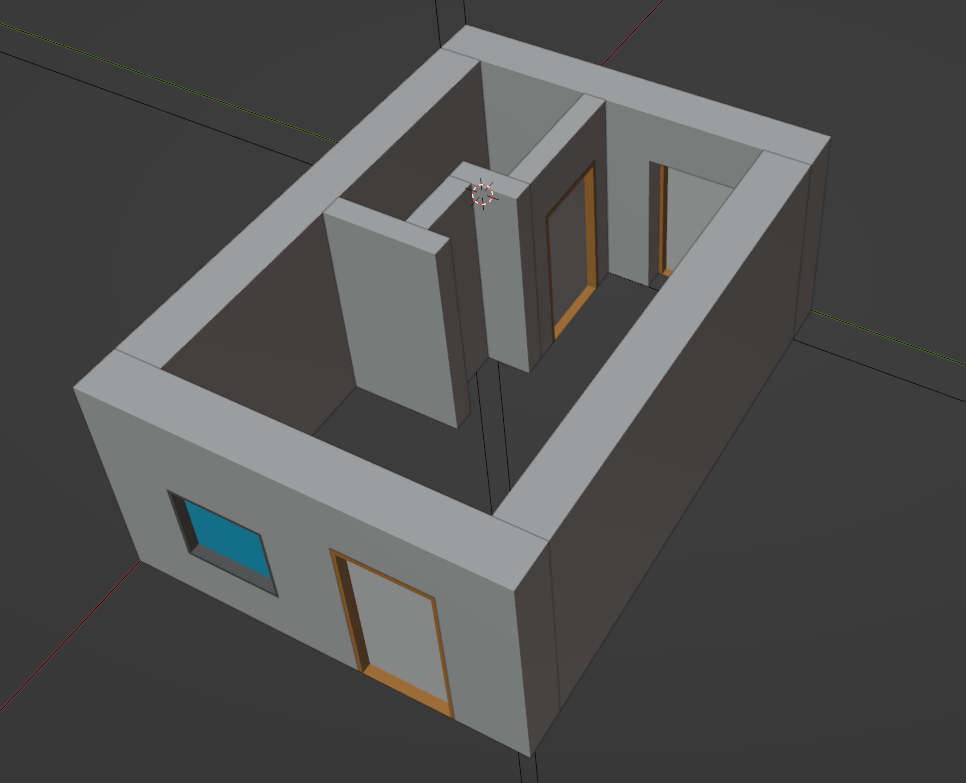
\includegraphics[width=0.5\columnwidth]{fig/scenario1_screenshot.png}
  \caption{TODO 3D Modell.}\label{fig:poc:scenario2 modell}
\end{figure}

\begin{figure}[ht!]
  \centering
  
\includegraphics[width=0.6\columnwidth]{fig/TODO.jpg}
  \caption{TODO Ergebnis Szenario 2.}\label{fig:poc:scenario2 ergebnis}
\end{figure}

\subsection{Szenario 3}\label{poc:scenario3}
\section{Regelbasierte Bauplandeduktion aus einem Bauplanentwurf}